\pdfminorversion=4

\documentclass[11pt]{beamer}
\usetheme{Copenhagen}
\usepackage[utf8]{inputenc}
\usepackage{amsmath}
\usepackage{amsfonts}
\usepackage{amssymb}
\usepackage{graphicx}
\usepackage{xcolor}
\usepackage{listings}
\author{Rodrigo Alejandro Melo - MLAB (ICTP) - CMNB (INTI)}
\title{The COMmunication BLOCK (Core ComBlock)}
%\setbeamercovered{transparent}
%\setbeamertemplate{navigation symbols}{}
%\logo{../images/header.png}
\institute{\tiny Advanced Workshop on Modern FPGA Based Technology for Scientific Computing | SMR 3289}
\date{May 20th, 2019}
%\subject{smr3289}
\begin{document}

\begin{frame}
  \titlepage
\end{frame}

\begin{frame}{Motivation}
  \begin{itemize}
    \scriptsize
    \item[•] MLAB projects are characterized by solving the high-speed processing in the FPGA and send the resulting data to a PC.
    \item[•] The Processor included in devices such as Zynq is mainly considered as a provider of data storage (DDR memory) and Ethernet connections.
    \item[•] The ComBlock was created to provide known interfaces (registers, RAM and FIFO) to a user of the Programmable Logic (PL), avoiding the complexity of the system bus provided by the Processor System (PS), which is AXI in case of the Zynq-7000.
  \end{itemize}
  \vspace{15mm}
  \begin{itemize}
    \scriptsize
    \item[•] The core ComBlock is a collaboration between the MLAB (ICTP) and the CMNB (INTI).
  \end{itemize}
\end{frame}

\begin{frame}{Features}
  \begin{columns}
    \column{0.3\textwidth}
      \center
      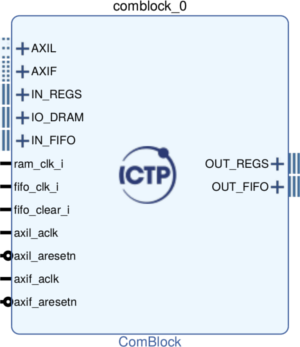
\includegraphics[width=1.0\textwidth]{../images/vivado/full.png}
    \column{0.7\textwidth}
      \begin{itemize}
        \tiny
        \item[•] Highly configurable: 5 interfaces with their own parameters.
        \item[•] 16 input and 16 output registers (configurable up to 32 bits).
        \item[•] A True Dual Port RAM, which provides a Simple RAM interface available to the user. Its inclusion, the data width, the address width and the memory depth can be configured.
        \item[•] Two asynchronous FIFOs, one from PL to PS and another from PS to PL, with indication of empty/full, almost empty/full and underflow/overflow conditions. Their individual inclusion, the data width and the memory depth can be configured.
        \item[•] In the Vivado version, an AXI Lite interface was used for the registers and AXI Full interfaces for the RAM and FIFOs.
      \end{itemize}
  \end{columns}
  \vspace{5mm}
  \scriptsize
  Under the hood, it was descripted using VHDL'93 and inferred memories of the FPGALIB project (\url{https://github.com/INTI-CMNB-FPGA/fpga_lib}), which were tested with Xilinx, Intel/Altera and Microsemi devices.
\end{frame}

\begin{frame}{How to get}
  \begin{itemize}
    \scriptsize
    \item[•] Gitlab repository \url{https://gitlab.com/rodrigomelo9/core-comblock}
    \item[•] You can clone it (Git)
    \item[•] Or you can download it (compressed)
  \end{itemize}
  \center
  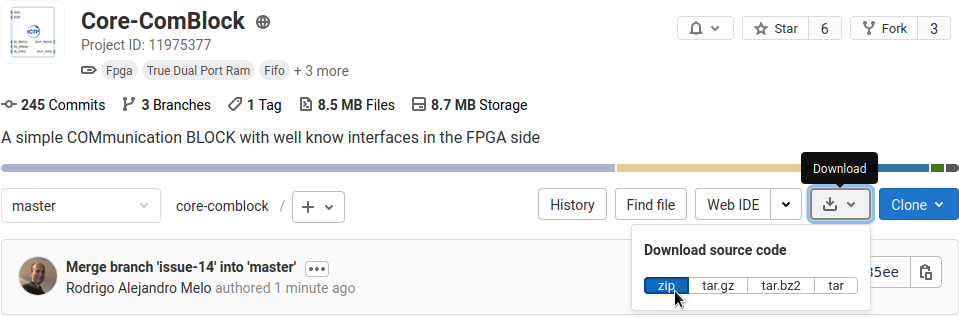
\includegraphics[width=\textwidth]{../images/repo.png}
  \begin{itemize}
    \scriptsize
    \item[•] It is licensed under the BSD 3-clause.
  \end{itemize}
\end{frame}

\begin{frame}{How to add to Vivado}
  \begin{itemize}
    \scriptsize
    \item[•] Flow Navigator $\rightarrow$ Project Settings
    \item[•] IP $\rightarrow$ Repository
    \item[•] Add Repository button (+)
    \item[•] Browse to \textit{COMBLOCK\_ROOT\_PATH/ip\_repo}
  \end{itemize}
  \center
  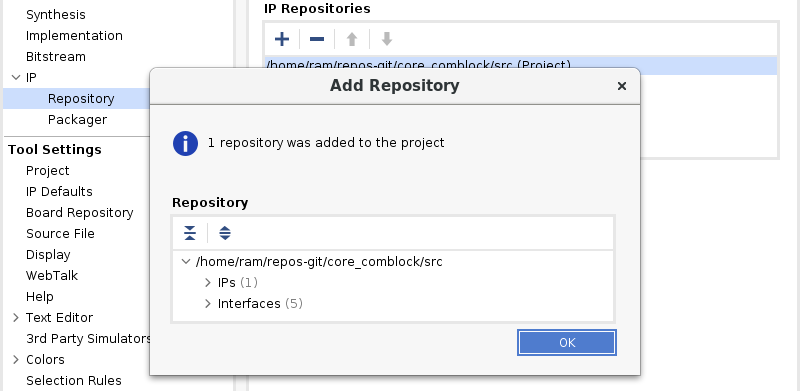
\includegraphics[width=0.5\textwidth]{../images/vivado/add-repo.png} \\
  \scriptsize
  Note: the five interfaces in the image are internally used by the core.
\end{frame}

\begin{frame}{Customizations}
  \center
  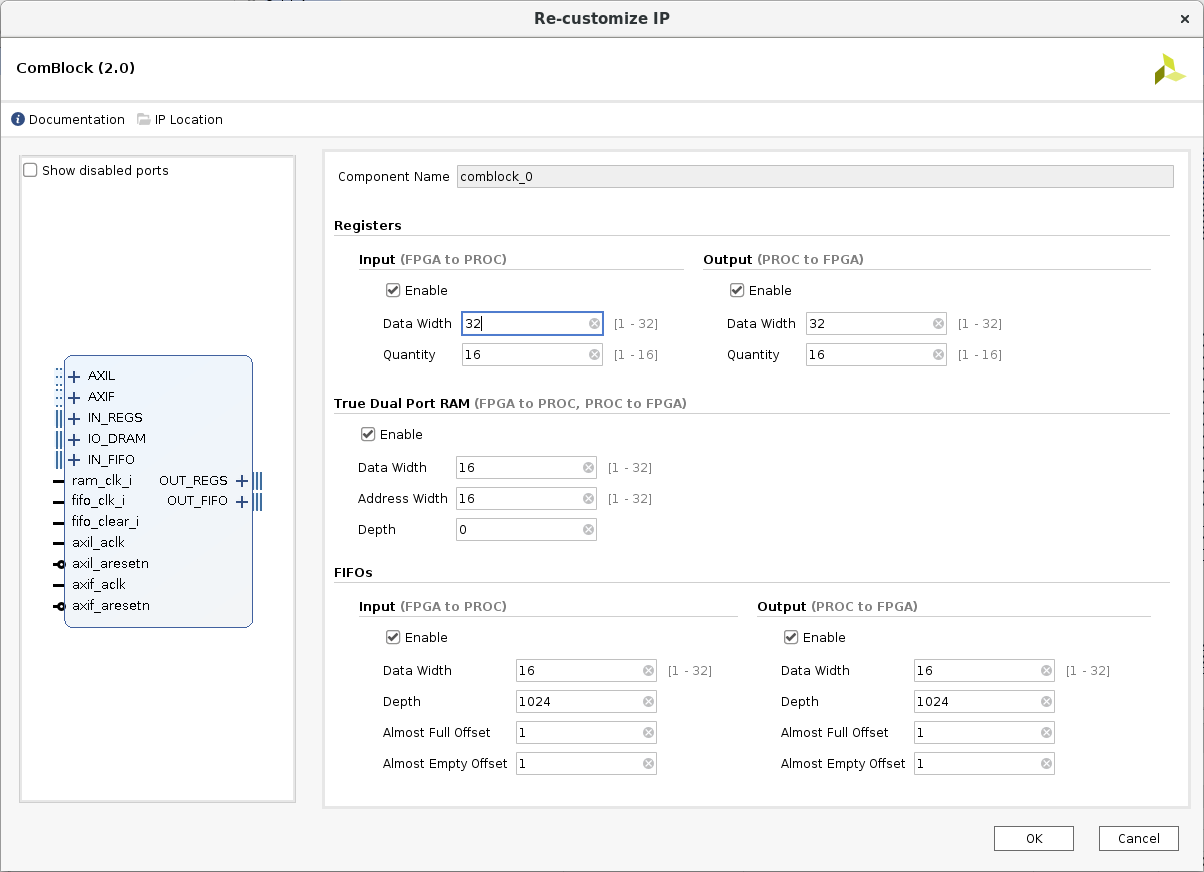
\includegraphics[width=0.95\textwidth]{../images/vivado/config.png}
\end{frame}

\begin{frame}{Registers}
  \begin{columns}
    \column{0.4\textwidth}
      \center
      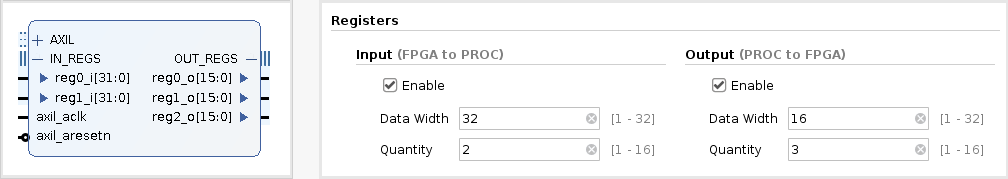
\includegraphics[width=\textwidth]{../images/vivado/only-regs.png}
    \column{0.6\textwidth}
      \begin{itemize}
        \scriptsize
        \item[•] The output register are automatically active when the other interfaces are disabled
        \item[•] Input and Output registers are Read/Written from 0 to 15
        \item[•] Output registers can be also Read/Written from 16 to 31
      \end{itemize}
    \end{columns}
\end{frame}

\begin{frame}{True Dual Port RAM}
  \begin{columns}
    \column{0.6\textwidth}
      \begin{itemize}
        \scriptsize
        \item[•] The True Dual Port RAM Interface is considered as I/O (bidirectional)
        \item[•] If DEPTH is 0, the quantity of memory positions is calculated as 2**AWIDTH
        \item[•] A DEPTH greater than 0 is useful when the complete address space produce a waste of resources (as example, in the Xilinx 7-series, the BRAM are used as 18/36 Kb, which are not a power of 2)
      \end{itemize}
    \column{0.4\textwidth}
      \center
      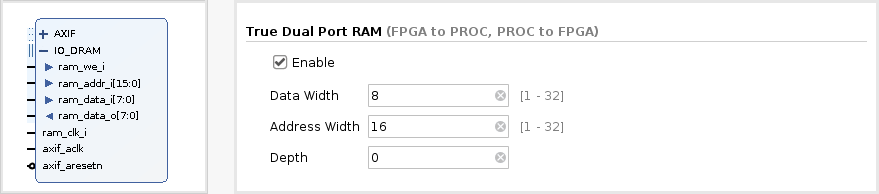
\includegraphics[width=\textwidth]{../images/vivado/only-dram.png}
    \end{columns}
\end{frame}

\begin{frame}{FIFOs}
  \begin{columns}
    \column{0.4\textwidth}
      \center
      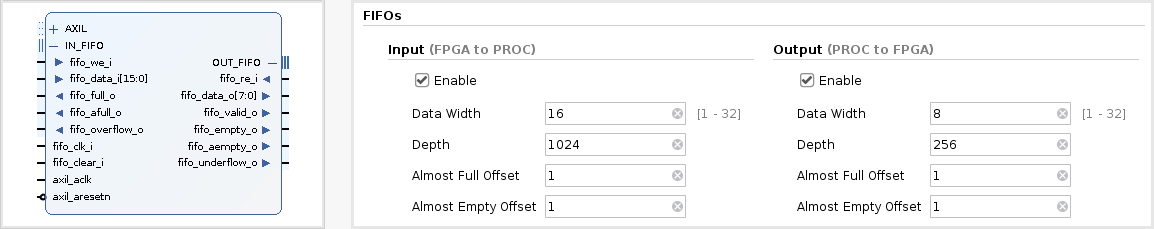
\includegraphics[width=\textwidth]{../images/vivado/only-fifos.png}
    \column{0.6\textwidth}
      \begin{itemize}
        \scriptsize
        \item[•] Both FIFOs are asynchronous
        \item[•] The FIFO was designed to work in a conservative way
        \item[•] The Clear input is used to have a know state
        \item[•] DEPTH has the same sense that in the DRAM\_IO interface
        \item[•] AEMPTY and AFULL means \textit{Almost}
      \end{itemize}
    \end{columns}
\end{frame}

\begin{frame}[fragile]{C Driver}
  \begin{itemize}
    \scriptsize
    \item[•] If you used the ComBlock in your block design, you can add:
      \begin{lstlisting}[language=C, numbers=none]
#include "comblock.h"
      \end{lstlisting}
    \item[•] It has some defines:
      \begin{lstlisting}[language=C, numbers=none]
...
#define COMBLOCK_IREG11 11*4
...
#define COMBLOCK_OREG9  25*4
...
      \end{lstlisting}
    \item[•] And functions to make discrete read/write operations:
      \begin{lstlisting}[language=C, numbers=none]
...
static inline void ComBlock_Write(UINTPTR Addr, u32 Value) {
...
static inline u32 ComBlock_Read(UINTPTR Addr) {
...
      \end{lstlisting}
  \end{itemize}
\end{frame}

\begin{frame}[fragile]{How to Read/Write}
  \begin{itemize}
    \scriptsize
    \item[•] In \textit{xparameters.h} you can found something like:
      \begin{lstlisting}[language=C, numbers=none, basicstyle=\tiny]
#define XPAR_COMBLOCK_0_AXIL_REGS_BASEADDR 0x43C00000
#define XPAR_COMBLOCK_0_AXIF_DRAM_BASEADDR 0x7AA00000
#define XPAR_COMBLOCK_0_AXIF_FIFO_BASEADDR 0x7AA10000
      \end{lstlisting}
    \item[•] In \textit{xil\_io.h} you have functions to read and write:
      \begin{lstlisting}[language=C, numbers=none, basicstyle=\tiny]
static INLINE Xil_In32(UINTPTR Addr) // Also 8, 16 and 32
static INLINE void Xil_Out32(UINTPTR Addr, u32 Value) // Also 8, 16 and 32
      \end{lstlisting}
    \item[•] Also yoy can use the memcpy function:
      \begin{lstlisting}[language=C, numbers=none, basicstyle=\tiny]
void *memcpy(void *str1, const void *str2, size_t n)
      \end{lstlisting}
    \item[•] And the functions of the driver.
  \end{itemize}
\end{frame}

\begin{frame}[fragile]{Examples}
  \begin{itemize}
    \scriptsize
    \item[•] Registers:
      \begin{lstlisting}[language=C, numbers=none, basicstyle=\tiny]
ComBlock_Write(XPAR_COMBLOCK_0_AXIL_REGS_BASEADDR+COMBLOCK_OREG1,0x99);
value = Xil_In32(XPAR_COMBLOCK_0_AXIL_REGS_BASEADDR+8*4);
      \end{lstlisting}
    \item[•] FIFOs:
      \begin{lstlisting}[language=C, numbers=none, basicstyle=\tiny]
value = ComBlock_Read(XPAR_COMBLOCK_0_AXIF_FIFO_BASEADDR);
      \end{lstlisting}
    \item[•] DRAM:
      \begin{lstlisting}[language=C, numbers=none, basicstyle=\tiny]
memcpy(buffer,(UINTPTR *)XPAR_COMBLOCK_0_AXIF_DRAM_BASEADDR,SAMPLES*sizeof(int));
memcpy((UINTPTR *)XPAR_COMBLOCK_0_AXIF_DRAM_BASEADDR,buffer,SAMPLES*sizeof(int));
for (i = 0, i < SAMPLES; i++)
    Xil_Out32(XPAR_COMBLOCK_0_AXIF_DRAM_BASEADDR+i*4, 1234);
      \end{lstlisting}
  \end{itemize}
\end{frame}

\begin{frame}{Roadmap}
  \begin{itemize}
    \scriptsize
    \item[•] Add support to more devices:
      \begin{itemize}
        \scriptsize
        \item[•] Zynq UltraScale+
        \item[•] Intel/Altera Cyclone V + SoC
        \item[•] SmartFusion2
        \item[•] PolarFire + RISC-V
      \end{itemize}
    \item[•] Add special registers (and functions) to read the hardware configuration from the PS.
    \item[•] Add an optional AXI4-Stream High Speed Interface to the FIFOs.
    \item[•] Add functions to drive the DRAM interface using memcpy.
  \end{itemize}
\end{frame}

\end{document}
